\label{chap:design}
As Futhark focuses on producing efficient parallel code, it also imposes
constraint on the language semantics, in order to do so. 
These constrains will in turn impose limitations on the design of the library,
where the most significant limitations are that arrays cannot be irregular and
cannot hold function types. 
Without these limitations we could define a network as an array of layers each
containing a set of functions and weights. 
Forward and backward passes could then be performed by a \texttt{fold}-like
operation, which would be the approach in any other functional language, 
but unfortunately not possible in Futhark. We therefore need to look for
alternative solutions.
\section{Design}

The initial solution was to split layer functions and weights into two separate
parts, which would avoid the two limitations mentioned above. 
As layers in a neural network have different sizes, the limitation of irregular
arrays, makes a natural one-to-one array representation of weights impossible. 
To overcome this my initial design used a weight representation of a
one-dimensional array, but this required the need for additional information of
indexes, to keep track of which weight slices belongs to which layers. 
Furthermore, additional information was required, such as the layer type, weight
shape, activation functions etc., for each layer in the network, where layer
type and activation functions where defined by integer values. 
The idea was that depending on the layer type, the appropriate layer logic would
be applied to handle, for instance the forward pass for a fully-connected layer.

I could then define a network as \texttt{type nn =  (weights,
	layer\_information)}. 
The separation of weights and layer functions meant that we needed a function
with some control structure to perform a forward and backward pass for a
network. 
The pseudo-code in Algorithm \ref{algo} shows such a function for the forward
pass.  
\begin{algorithm}[!htbp]
	\caption{Forward propagation}
	\begin{algorithmic}[1]
		\Procedure{Forward propagation}{input, nn}
		\For    {l in nn.layer\_information}
		\State  (activation, dims, weight\_indexs) $\gets$ l    // Extract layer
		information
		\State  weights\_flat $\gets$ nn.weights[weights\_indexs]
		\State  weights $\gets$ \texttt{reshape} dims weights\_flat
		\State  output $\gets$ apply weights and activation to input
		\State  input $\gets$ output // Write output to input for next layer  
		\EndFor
		\Return output
		\EndProcedure
	\end{algorithmic}
	\label{algo}
\end{algorithm} 
This would be the approach in most imperative languages and at first sight seems
reasonable in Futhark as well. 
But one main optimization in implementing the backpropagation algorithm
efficiently, is to store information produced during the forward pass for the
backward pass to avoid recomputing results. 
These can only be stored as a one-dimensional array, because of the non-regular
sizes of layers, and would again require an additional set of indices. 
The general problem with this representation is that the restriction on
non-regular arrays, means that most data needs to be stored as one-dimensional
arrays, with a corresponding set of indices and shape parameters. 
Every time a layer needs to perform an operation, it first needs to extract the
data and reshape it. 
While reshaping might not result in compute-intensive operations, it is an
unfortunate consequence of this representation. 
The additional set of indices and shape dimensions creates a library that uses
additional information and operations, which can be avoided in most other
languages. Thus using an array representation of a network in Futhark is not an
optimal solution. 
Additionally as weights and layer logic is separated, dependencies would be
scattered all over the library and extending it would require changes in several
places, which will inevitably hinder the maintainability. 
Splitting weights and layer logic is therefore not a viable solution either.
\newline \newline 
Recall from Section \ref{sec:forward} that the network was combined by letting
the output of the first layer be the input to next one and that we can express a
neural network as a function, that takes some weights and input and returns some
output. 
From the derivation of the backpropagation algorithm, we saw that the errors
from the output layer was passed back through the network, where each layer
passes errors to the previous one. 
Using these observations, we can view a neural network as two main
functions(i.e., for a network of depth $n$ we can write
$f_n(f_{n-1}(\cdots(f_1(\cdot)))$ for the forward pass and likewise for the
backward pass $b_1(b_{2}(\cdots(b_n(\cdot ))))$). 
This is the main idea behind this implementation, where neural networks are
represented as a composition of functions. 
With this representation, a single layer is now essentially the same as a
one-layer network, which defines two functions $f(\cdot)$ and $b(\cdot)$. 
Conceptually the idea is simple, but the functions need to carry some additional
information for this idea to be implemented efficiently. 
Therefore we need to define abstract functions that can do so:
\begin{lstlisting}[caption={Auxiliary abstract types for specifying neural
networks},language=futhark, numbers = left]
type forwards   'input 'w 'output 'cache = 
bool $\to$ w $\to$ input $\to$ (cache, output)
type backwards   'w  'cache 'err_in  'err_out '^u = 
bool $\to$ u $\to$ w $\to$ cache $\to$ err_in $\to$
(err_out, w)
\end{lstlisting}
where $'$(apostrophe) means that \emph{input, w, output, cache}, and so on, are
abstract types and 
\ $\widehat{\ }\ $\  means that $u$ is a functional type (and also abstract
because of the apostrophe).
The abstract semantics of the functions are:
\begin{itemize}
	\item \texttt{forwards:} Values of this type take, a boolean, some weights, and
	input and returns a cache and the output from the network. 
	The cache stores intermediate results, such that when we backpropagate we do
	not have to recompue the values. 
	The boolean argument is there to indicate if the function is called during
	training; if it is not, then we can just return an empty cache. 
	
	\item \texttt{backwards:} Values of this type take, a function $u$ for applying
	the gradients to the weights, some weights, the information stored in the cache
	from the forward pass, and the errors that are backpropagated from the above
	layer. 
	The returned value is the updated weights and the errors that is backpropagated
	further down the network. 
	The function $u$ is provided by the type of optimizer that is used, e.g.
	gradient descent, which enables the handling of gradients in different ways. 
	Other types of optimizers can then be implemented later on through the function
	$u$.
	
	The boolean is there to indicate if it is the first layer of the network, and
	if it is, then we do not need to calculate and backpropagate the error. 
	This is a small optimization, but can give a performance increase on longer
	training passes.
	
\end{itemize}
As these are fully abstract function types,  means that a layer implementation
needs to define it's own concrete types, but note that, how one layer chooses
it's concrete types will affect if the layer can be combined with other layer
types, which in some cases will require an utility layer. 
In the implementation we require a layer to supply  these two functions with the
abstract semantics above, but the internal logic is defined by the layer it
self. 
Additionally must the layer also define and possibly provide some weights. 
Combining it all we can write the complete network type as:
\begin{lstlisting}[language=futhark, caption = {Abstract type for representing a
neural network}]
type NN 'input 'w 'output 'c 'e_in 'e_out '^u =
{ forward : forwards input w output c,
backward: backwards c w e_in e_out u,
weights : w }
\end{lstlisting}
In the implementation I'm using a more concrete function in the network type
instead of the abstract function $u$:
\begin{lstlisting}[language=futhark, numbers = left, caption = {Function
signature for applying gradient}]
--- The weight definition used by optimizers
type std_weights 't = ([][]t, []t)
type apply_grad 't  = std_weights t $\to$ std_weights t $\to$ std_weights t
\end{lstlisting} 
As optimizers have to operate on the weights and gradients, they need to know
its concrete type, and therefore the abstract function \texttt{apply\_grad} with
a concrete signature is used. 
Layers that do not use this weight representation needs to reshape their weights
and gradients before applying the function. 
Most optimizers update gradients and weights in bulk operations (e.g. all
gradients gets the same learning rate applied), and therefore will reshaping not
affect the update, but if some optimizer does not treat gradients in bulk, then
this design may be a non-optimal. \newline   \newline  
Networks can be combined by using the core function of the library
\texttt{connect\_layers}, which takes two networks and combines them into one
through lambda expressions. 
\begin{lstlisting}[language=futhark, caption = {Function for combining two
networks}, label = {connect}]
let connect_layers 'w1 'w2 'i 'o1 'o2 'c1 'c2 'e1 'e2 'e
({forward=f1, backward=b1,
weights=ws1}: NN i w1 o1 c1 e e1 (apply_grad t))
({forward=f2, backward=b2,
weights=ws2}: NN o1 w2 o2 c2 e2 e (apply_grad t))
: NN i1 (w1,w2) (o2) (c1,c2) (e2) (e1) (apply_grad t) =

{forward = \(is_training) (w1, w2) (input) ->
let (c1, res)  = f1 is_training w1 input
let (c2, res2) = f2 is_training w2 res
in ((c1, c2), res2),

backward = \(_) u (w1,w2) (c1,c2) (error) ->
let (err2, w2') = b2 false u w2 c2 error
let (err1, w1') = b1 true u w1 c1 err2
in (err1, (w1', w2')),

weights = (ws1, ws2)}
\end{lstlisting}
The forward functions are straightforwardly combined and like so for the
backward functions, just in reverse order. 
As mentioned above, there are some type restrictions when combining two
networks, $nn_1$ and $nn_2$. 
The output type of $nn_1$ {must} match the input type of $nn_2$ {and} the error
output type of $nn_2$ must match the error input type of $nn_1$, which are the
only restrictions when connecting two networks. 
These restriction are also reflected in the two neural network types in Listing
\ref{connect}, (e.g. the output type from the first network, $o1$ on line 3 is
the same as the input to the second network on line 5). 
Weights and caches are also combined into tuples, becoming more and more nested
as the network depth increases. 
The tuples are then unfolded when functions are called deeper into a multilayer
network. 
This representation completely avoids the use of 1-dimensional arrays and
indexing, but instead inline functions and make use of tuples to represent a
network. 
We can store information in their correct form and also avoid storing auxiliary
information. 
Additionally, extending the library with a new layer, is only limited to the
concrete layer implementation itself and does not affect other parts. 
Such a representation is clearly favored and is also more natural to the
definition of a neural network. 

\section{Library structure}
Having defined the core types and functions of the library, this section will
provide an overview of the library structure. 
The implementation makes use of the ML-style module system in Futhark. 
As a neural network consists of many components, we naturally should separate
each of these into their own modules. 
Weight initialization- , activation- and loss functions are implemented within
their own modules respectively. 
Layer implementations are a bit different, where I define a module type (i.e. an
abstract module) \emph{layer\_type}, which each concrete layer implementation
uses. 
Each concrete layer implementation is then collected in the module
\emph{layers}, such that we can access all of the layers through a single
module. Optimizer implementations follow the same structure as layers. 
As layers and optimizers in general have more complex implementations, using a
level of abstraction is needed. 
Lastly is the \emph{neural\_network} module, where the \texttt{connect\_layers}
function is implemented. 
This module contains more generic utility functions, such as functions for
calculating the loss or accuracy of a network. 
The next sections will provide details on the implementations, starting with
activation functions. 


\section{Activation functions}
Recall that an activation function has the characteristic of being
\emph{differentiable}, such that, we can use it's derivative during the backward
pass in order to calculate the gradient. 
Therefore are activation functions represented as a pair, containing the
function it self and it's derivative, i.e. we can define it's abstract type as
\begin{lstlisting}[language=futhark, caption = {Abstract activation function
type}]
type activation_func 'o = {f:o $\to$ o, fd:o $\to$ o}
\end{lstlisting}
The activation functions provided in this implementation all use a 1-dimensional
array as their concrete type, which is required since the softmax function is
applied on a sequence of activations. 
A key reason for this representation is that the user can define their
\emph{own} pair of functions and use them should the library not contain them.
This ensures a flexible system, where the user is not limited to the library
implementation. 
Supported activation functions are \emph{sigmoid, tanh, ReLU, identity} and
\emph{softmax}, though softmax can not be used during training in a
layer\footnote{See Section \ref{shortcoming} for more details}. 
The implementations follows the definitions given in Table \ref{tab:activation}
and only softmax has been implemented differently by subtracting the maximum
value on each element, before applying the exponential function such that
overflowing is avoided. 
The activation functions can be accessed through the \emph{neural\_network}
module through simple wrappers, following the same interface as Tensorflow.
\section{Loss function}
The definition of loss functions follows the same idea as activation functions,
but they just have a different signature. 
\begin{lstlisting}[language=futhark, caption = {Abstract loss function type}]
type loss_func 'o  't   = {f:o $\to$ o $\to$ t, fd:o $\to$ o $\to$ o}
\end{lstlisting}
Again, this allows users to define their own loss functions and in this
implementation a loss functions concrete type of  \ $'o$\   is a 1-dimensional
array. 
Supported loss functions are \emph{cross entropy, cross entropy with softmax}
and \emph{sum of squares}. 
The implementation of these follow the definitions given in Tabel
\ref{tab:loss}. \newline 

Both activation- and loss function types are defined globally as they are also
used by concrete layer modules and the \emph{neural\_network} module.

\section{Optimizers}
In this implementation optimizers performs the backpropagation algorithm, by
calling the forward and backward passes on a network and applies the gradients
through it's own implementation of the abstract function \texttt{apply\_grad}. 
In order to provide options on future implementations, optimizers are separated
with their own module type. 
The module type of an optimizer is defined as follows:
\begin{lstlisting}[language=futhark, caption = {Abstract optimizer module}]
module type optimizer_type = {
type t
type ^learning_rate
-- | Train function with signature
--   network $\to$ learning_rate $\to$ input data $\to$ labels $\to$ 
--   batch_size $\to$ loss function $\to$ 
--   Returns the same network with updated weights
val train 'i 'w 'g 'e2 'o : 
NN ([]i) w ([]o) g ([]o) e2 (apply_grad t)
$\to$ learning_rate 
$\to$ (input_data:[]i) 
$\to$ (labels:[]o) 
$\to$ i32 
$\to$ loss_func o t 
$\to$ NN ([]i) w ([]o) g ([]o) e2 (apply_grad t)
}
\end{lstlisting}
Where \emph{learning\_rate} is allowed to be a function type, which allows an
optimizer implementation to adapt the learning rate for different training steps
with a user defined function. 
The restrictions on the abstract function \texttt{train} is straightforward,
given a neural network, the input and output should match the input data and the
labels respectively. 
The input data and labels must be an array type, where each data point is an
element, such that we can easily loop through the input data. 
The loss function given as argument should also match the output type. 
The only optimizer the implementation provides is gradient descent defined in
the \emph{gradient\_descent} module. 
The process of training a network is performed by a loop:
\begin{lstlisting}[language=futhark, caption ={Train function in gradient
descent module}]
let train [n] 'w 'g 'o 'e2 'i (
{forward=f,
backward=b,
weights=w} : NN ([]i) w ([]o) g ([]o) e2 (apply_grad t))
(alpha:learning_rate)
(input:[n]i)
(labels:[n]o)
(batch_sz: i32)
({f=_, fd=loss'}:loss_func o t) =

let i = 0
let updater = apply_grad_gd alpha batch_sz

let (w',_) = loop (w, i) while i < length input do
let input'          = input[i:i+batch_sz]
let label'          = labels[i:i+batch_sz]
let (cache, output) = f true w (input')
let error           = map2 (\o l -> loss' o l) output label'
let (_, w')         = b false updater w cache error
in (w', i + batch_sz)
in {forward = f, backward = b,  weights = w'}


\end{lstlisting}
We forward propagate the input and calculate the error(line 17 and 18), which
are then backpropagated through the network to get the updated weights (line
18). 
The \texttt{updater} value is a function that takes the gradients and weights of
a layer and performs the update using equation (\ref{eq:update}). 
The process is repeated, until all of the given input data has been processed,
returning the same network with the updated weights. 

\section{Layers}
Recall that the errors are backpropagated back through the network using this
following equation for MLP:
\begin{equation}
\boldsymbol{\delta}^{(l)} = \underbrace{(W^{(l+1)})^T
	\boldsymbol{\delta}^{(l+1)}}_{error'}  \circ \ \sigma'^{(l)}(W^{(l)}
\boldsymbol{z}^{(l-1)} + B^{(l)})\\
\end{equation}
The \emph{error'} part is backpropagated in this implementation as the error
term, as it can be calculated at layer $l+1$, but not at layer $l$. 
The same part of the error term is used for a convolutional network. 
Recall also that when connecting a convolutional layer with a fully-connected
one, we'd need to swap this exact part. 
Therefore must the layer implementations follow this convention, such that we
can backpropagate the errors correctly. 
The remaining part, $\sigma'_{(i)}(W^{(l)} \boldsymbol{z}^{(l-1)} + B^{(l)})$ is
calculated at layer $l$, where $W^{(l)} \boldsymbol{z}^{(l-1)} + B^{(l)}$ is
retrieved from the cache. 
The abstract layer module \emph{layer\_type} is defined as:
\begin{lstlisting}[language=futhark, caption = {Abstract layer module}]
module type layer_type = {
type t
type input_params
type ^activations

type input
type output
type weights
type err_in
type err_out
type cache
-- Initialize layer given input params, 
-- activation func and seed
val init: input_params -> activations -> i32 -> 
NN input weights output cache err_in err_out (apply_grad t)
}
\end{lstlisting}
Thus a concrete layer implementation must define it's own \emph{input, output,
	weights, err\_in, err\_out}, and \emph{cache} types and must provide a function,
that initializes the layer given its own defined input parameters and 
activation function. 
The integer given is used as a seed parameter, which is used for layers with
weight initialization. 
Note that layer functions are expecting a batch of data points at the time for
forward and backward passes, such that the parallelism is optimized. \newline
\newline 
The implemented layers are \emph{dense \text{(fully-connected)}, 2D
	convolutional, max-pooling}, and \emph{flatten}. 
The latter is a utility layer, which allows a convolutional layer to be combined
with a dense one. 
\subsection{Dense}
The dense layer is initialized with a tuple of two integers, $(m,n)$, which
represents the input and output dimensions respectively. 
The weights are then represented as a matrix of dimensions $n \times m$, where
each row represents the weights associated with a neuron, along with a
1-dimensional array of length $n$ for the biases, following the same
representation as in Section \ref{sec:forward}. 
The forward pass is implemented one-to-one using equation (\ref{eq:forwardmlp}),
with appropriate transposing of the input data, as it is in row format. 
Matrix multiplication is performed using the function \texttt{matmul} from the
\texttt{futlib/linalg} library. 
The cache in a dense layer consists of the original input and the result after
applying the biases, which are used during backpropagation. 
The backward pass is implemented using equation (\ref{eq:backwardmlp}),
(\ref{eq:backpropwmlp}) and (\ref{eq:backpropBias}) directly. 

\subsection{Convolutional}
The implementation of a convolutional layer is not as straightforward as the
dense one. 
There are many ways convolutions can be implemented efficiently today, with each
method having different strengths and weaknesses. 
The need for performing fast convolution is evident in that convolutional
networks are used in real-time applications such as self-driving cars for
detecting pedestrian, which requires low latency, so the success of a
convolutional network is limited by how fast we can perform the convolution
\cite{DBLP:journals/corr/Lavin15b}. 
Convolutional operations are compute-expensive operations and H. Kim et. al.
\cite{Performance} show that more than 70\% of the training time is spent in
convolutional layers on the AlexNet network, which consists of 5 convolutional
layers and 4 fully-connected layers. 
The search for faster convolutional algorithms is still an active area of
research, where the common approach is to reduce the amount of multiplication
operations at the expense of additions and/or use of auxiliary memory. 

The simplest way is to implement the convolutional operation directly, following
equation (\ref{eq:directconv}), but this also leads to very slow performance. 
Another approach is to lower the convolution into a matrix multiplication, which
can be done by transforming image data into matrices using a function called
\texttt{im2col}, which arranges the image slices into a column matrix. 
This is also called the GEneric Matrix-Matrix multiplication (GEMM) approach. 
By representing filters as matrices as well, we can perform the convolutional
operation as a matrix multiplication. Matrix multiplication can be done very
efficiently on GPUs, as it can utilize the local memory that has low latency and
high bandwith. 
The downside is that it uses a lot of auxiliary memory and also additional
resources to transform the data to matrix form. 
As an example given a $4 \times 4$ image and a filter of size $2\times 2$ with a
stride of 1, Figure \ref{im2col} shows how the transformation duplicates the
data by a factor of 2.25. This factor increases linearly with the image size,
fixing everything else.  
\begin{figure}[!hbtp]
	\begin{displaymath}
	\begin{bmatrix}
	x_{00} & x_{01} & x_{02} & x_{03} \\ 
	x_{10} & x_{11} & x_{12} & x_{13} \\ 
	x_{20} & x_{21} & x_{22} & x_{23} \\ 
	x_{30} & x_{31} & x_{32} & x_{33}  \\  
	\end{bmatrix}
	\underbrace{\Rightarrow}_{\text{im2col}}
	\begin{bmatrix} 
	x_{00} & x_{01} & x_{02} & x_{10} & x_{11} & x_{12} & x_{20} & x_{21} & x_{22}
	\\ 
	x_{01} & x_{02} & x_{03} & x_{11} & x_{12} & x_{13} & x_{21} & x_{22} & x_{23}
	\\
	x_{10} & x_{11} & x_{12} & x_{20} & x_{21} & x_{22} & x_{30} & x_{31} & x_{32}
	\\ 
	x_{11} & x_{12} & x_{13} & x_{21} & x_{22} & x_{23} & x_{31} & x_{32} & x_{33}
	\end{bmatrix}
	\end{displaymath}
	\caption{Example of $im2col$ operation on a $4\times 4$ image with a $2 \times
		2$ filter and stride of 1}
	\label{im2col}
\end{figure} \newline
The Fast Fourier Transformation (FFT) along with the convolution theorem is
another popular approach \cite{DBLP:journals/corr/VasilacheJMCPL14}, but this
approach only performs well for large filter sizes as the extra padding on small
filters and unused calculations outweighs the benefit of performing element-wise
multiplications. 
It also only works with a stride equal to one \cite[p. 59]{Performance}. 
For filters of smaller sizes, 5 and below, the Winograd minimal filtering (WMF)
\cite{DBLP:journals/corr/Lavin15b} algorithm is usually better than FFT. 
The WMF algorithm is also based on the GEMM approach and achieves its
performance gain by transforming the data with pre-computed auxiliary matrices,
for each filter size, which reduces the arithmetic complexity of the
convolutional operation. 
Because of these matrices needs to be pre-computed means that each filter size
requires a special case and therefore is the WMF algorithm only applicable to a
small set of filter sizes. The two latter methods also uses excess amount of
auxiliary memory to hold intermediate results. \newline \newline 
Note that determining which algorithm is fastest cannot always be predetermined,
as it also depends on batch size, stride, and on. 
For example, Tensorflow executes all available algorithms, to figure out which
is best \cite[p. 60]{Performance}. cudNN \cite{nvidia} have all three approaches
implemented into their library, but clearly implementing all three algorithms is
a huge task and not feasible in this project. 
As both FFT and WMF algorithms doesn't apply for a general convolutional layer,
these algorithms have been neglected for now.  \newline \newline 
This leaves us with one last option, which is to use the GEMM approach, which
can be applied in the general case. H. Kim et. al \cite{Performance} (see Figure
\ref{fig:performance}) show that the GEMM approach performs reasonably well for
small batch sizes, but scales poorly as the batch sizes increases, because the
transformation to matrix form becomes too expensive.
\begin{figure}[!htbp]
	\centering
	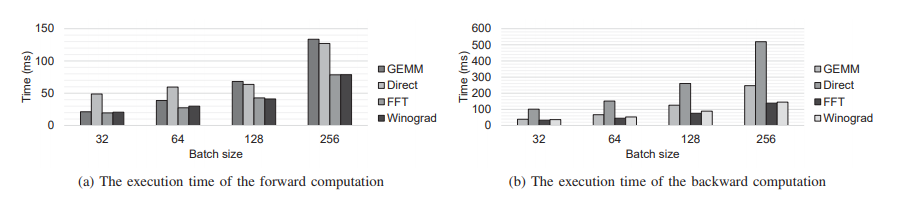
\includegraphics[width=\textwidth]{pics/performance}
	\caption{Performance comparison on forward and backward passes between  Direct
		convolution, GEMM, FFT and WMF algorithm on the AlexNet (source:
		\cite{Performance})}
	\label{fig:performance}
\end{figure}\newline 
The auxiliary memory usage can also become an issue and caused memory allocation
failures on a NVIDIA GTX 970 with 4GB of memory. 
The cudNN library solves this by reading fixed sized sub matrices of the input
data from the off-chip memory onto the on-chip memory successively and computes
a subset of the output. 
This is done while fetching the \emph{next} sub matrices onto the on-chip
memory, essentially hiding the memory latency associated with the data transfer,
thus is the computation only limited by the time it takes to perform the
arithmetic, while limiting the auxiliary memory usage\cite[p.
5]{DBLP:journals/corr/ChetlurWVCTCS14}. 
The cudNN library provide both options in their API (i.e. to form the matrix
explicitly or implicitly). 
Interestingly enough, \cite{Performance} shows that the GEMM method has a less
or equal peak memory usage than direct convolution, though it is not clear which
GEMM method is used in the paper, but assuming that the explicit method is used,
since they have $4 \times 12GB$ of GPU memory and the showed peak memory usage
is below 6GB. 
The same result was also encountered in practice\footnote{There is an
	experimental implementation on branch 'directconv', which uses direct
	convolution, but the implementation is rather messy and no longer maintained},
where the direct convolution not only had worse performance, but got memory
allocation failures at fewer data points. 
The exact reason for this is unknown, but it seems that the GEMM method is
superior to direct convolution in terms of performance and memory usage. 

The implicit GEMM approach is not possible in Futhark, and the closest approach
is to perform a loop, which iterate through the input, computing each in chunks,
but this approach does not hide the memory latency and seems like a half
solution to the problem, as different systems have different memory capacities. 
As the  memory allocation failures only occur, when calculating the accuracy for
many data points at the same time, well above the normal batch sizes used during
training, the implicit method has been skipped in this work, but consider this
future work to find an alternative solution. \newline 
Therefore have the explicit GEMM approach been implemented, which transforms the
input image into matrix form explicitly.

\subsubsection{Implementation}
The convolutional layer implementation takes four parameters, \emph{number of
	filters}, \emph{filter size}, \emph{stride}, and \emph{input depth}. 
The latter is needed to initialize the proper filter depth to match the input
depth. 
Note that it is only possible to have square filters, but as it is the most
common, it is not a big issue, but extending it to allow for non-square filter
sizes is not difficult. 
The input layout for $N$ images is assumed to be $N \times D \times H \times W$,
where $D,H$ and $W$ is depth, height, and width respectively. 

\subsubsection*{Forward pass}
The forward pass is done by using the \texttt{im2col} function, which transforms
the image given filter size and image offsets into a matrix. 
By representing filters as a matrix and with the image matrix in place the
convolutional operation can be performed by a matrix multiplication. 
The biases and the activation function is then applied to the result. 
\begin{figure}[!hbtp]
	\begin{displaymath}
	\begin{bmatrix}
	f_{0,0,0} & f_{0,1,0} \\ 
	f_{1,0,0} & f_{1,1,0}  \\  
	\end{bmatrix}
	\begin{bmatrix}
	f_{0,0,1} & f_{0,1,1} \\ 
	f_{1,0,1} & f_{1,1,1}  \\  
	\end{bmatrix}
	{\Rightarrow}
	\begin{bmatrix}
	f_{0,0,0} & f_{0,1,0} & f_{1,0,0} & f_{1,1,0} & f_{0,0,1} & f_{0,1,1} &
	f_{1,0,1} & f_{1,1,1}    
	\end{bmatrix}
	\end{displaymath}
	\caption{A single filter of size $2 \times 2 \times 2$ representation in a
		convolutional layer}
	\label{fig:filter}
\end{figure} \newline 
The cache consists of the image matrix, which avoids doing the transformation
again during the backward pass, but we need to store the original image
dimensions additionally. 
We also cache the result of the convolutional operation after applying the bias
in the \emph{correct} format, such that we do not have to reshape it when we
perform the Hadamard product during backpropagation. 
\subsubsection{Backward pass}
The backward pass is based on equations (\ref{eq:backwadconvdelta}) and
(\ref{eq:backwadconv}). Having calculated $\boldsymbol{\delta}^{(l)}$, we need
to flatten each of the layers, to be able to perform a matrix multiplication for
the convolutional operation in (\ref{eq:backwadconv}) with the image matrix from
the cache.
For backpropagation of the errors to the previous layer, we need to flip the
filters first, which can be done by slicing into the filter vector and reverse
each filter separately using the Futhark function \texttt{reverse}. 
\begin{figure}[!hbtp]
	\begin{displaymath}
	\begin{bmatrix}
	f_{1,1,0} & f_{1,0,0} & f_{0,1,0} & f_{0,0,0} & f_{1,1,1} & f_{1,0,1} &
	f_{0,1,1} & f_{0,0,1}
	\end{bmatrix}
	\end{displaymath}
	\caption{Flipped filter from Figure \ref{fig:filter}.}
\end{figure} \newline 
Recall that equation (\ref{eq:backwadconvdelta}) is a full convolution and we
need to pad $\boldsymbol{\delta}^{(l)}$ before transforming it into matrix form.

From that representation we can perform a matrix multiplication again to perform
the convolutional operation.

\subsection{Max pooling}
A max pooling layer is initialized with a tuple of two integers, $(wm, wn)$,
which represents the dimensions of the sliding window, where the stride in the
two dimensions respectively is implied from those parameters. 
The forward pass is done by sliding the pooling window over the input image,
where each slice is given to the function \texttt{max\_val}, which returns the
index of the maximum value in the slice and the value itself as a tuple. 
The index is then transformed to an offset in the original image as if it was an
1-dimensional array and stored along with the maximum value. 
Lastly we unzip the offsets from the values and keep the offsets in the cache
and forward propagate the down-sampled values. 

The backward pass is done by using the offsets from the cache along with the
\texttt{scatter} function. 
The original image size is first created as a 1-dimensional array and filled
with zeros. 
Each of the 2-dimensional errors given is then flattened, and we can then
perform a \texttt{scatter} operation on each of them with the corresponding set
of offsets. 
Now every value is in the correct place and before returning, we reshape the
errors into the correct shape. 

\section{Weight initialization}
The Xavier initialization is implemented using the module
\textit{uniform\_real\_distribution}, which generates numbers from a uniform
distribution, from the Futhark library \texttt{futlib/random}. 
The Xavier initialization function is defined in the
\textit{weight\_initializer} module in the library. 
The implementation samples each number separately by generating a state from a
seed $s$. 
\begin{lstlisting}[caption = {Function for sampling a uniform number from the
seed $s$, by generating a state in line 2, which is used to sample the number in
line 3}, 	label = {rand} ]
let gen_rand_uni (s:i32)  (dist:(uni.num.t, uni.num.t)): t =
let rng = uni.engine.rng_from_seed [s]
let (_, x) = uni.rand dist rng in x
\end{lstlisting}
Normally you would only generate a single state for a sequence of random number,
where the state is updated and passed along for each call to \texttt{uni.rand}
in Listing \ref{rand}, but with this implementation the function can be called
with \texttt{map}, which allows one to generate the numbers in parallel, rather
than in a sequential order. The seeds given into the function
\texttt{gen\_rand\_uni} are generated through simple arithmetic, based on the
users chosen seed and requested weight dimensions.  The tests also show that the
numbers are sampled within the ranges provided by the distribution parameters,
which is sufficient. 
The initialization function are used by the \emph{dense} and
\emph{convolutional} layers, as they are the only ones with weights. 

\section{Additional network functions}
As we not only want to train a network, but also want to be able to evaluate a
model a number of additional functions are provided:
\begin{itemize}
	\item \texttt{predict}: Given a network, input data and an activation function,
	the \texttt{predict} function performs the forward pass of the network with the
	input data and returns the output activations.
	
	\item \texttt{accuracy}: The \texttt{accuracy} function takes a network, input
	data, labels and an activation function and performs the forward pass like
	\texttt{predict}, but additionally compares the output activations from the
	network with the labels. 
	The choice of comparison is done using either an \texttt{argmax} or
	\texttt{argmin} function\footnote{Recall from Chapter \ref{NN} that the output
		are interpreted as probabilities, and therefore will the output activation with
		highest probability be the prediction of the input. 
		The \texttt{argmin} comparison is usually used for cases, where the goal is
		predict, which is \emph{not} correct.}, which is given into the
	\texttt{accuracy} function as argument. 
	The function returns an percentage on how many data points the model correctly
	predicts, $\frac{\#hits}{\# data points}$. 
	
	\item \texttt{loss}: The function calculates the loss on a network given some
	input data, labels and a loss function. The accumulated loss of the input data
	and labels is returned. 
\end{itemize}
These functions are defined in the \emph{neural\_network} module. 

\section{Putting it all together}
The implementation defines a \emph{deep\_learning} module, which combines all of
the modules, \emph{layers}, \emph{optimizers}, \emph{loss} and
\emph{neural\_network} such that we only have to instantiate a single module. 
Having defined all of these components, we can now see how one can built the
convolutional network defined in Table \ref{table:conv2}  
\begin{table}[!htbp]
	\centering
	\begin{tabular}{|c|c|c|c|c|} \hline
		\textbf{Layer type} & \textbf{Filters/neurons} & \textbf{Filter/window size} &
		\textbf{Stride} & \textbf{Activation function} \\ \hline \hline 
		conv2d & 32 &  $5\times5$ & 1 & relu \\ \hline
		max pooling & 0 & $2\times2$ & 2 & N/A \\ \hline
		conv2d & 64 & $3\times3$ & 1 & relu \\ \hline
		max pooling & 0 & $2\times2$  & 2 & N/A \\ \hline
		dense & 1024  & N/A & N/A & identity \\ \hline
		dense & 10  & N/A & N/A & identity \\ \hline
	\end{tabular}
	\caption{Convolutional network with input dimension of $1 \times 28 \times 28$}
	\label{table:conv2}
\end{table}\newline 
The network in Table \ref{table:conv2} is build to be trained on the MNIST
data-set.
Listing \ref{network} show how we can put together such a network using the
library:
\begin{lstlisting}[language=futhark, caption = {Example of building a
convolutional network w. the library}, label = {network}]
import "../lib/deep_learning"
module dl = deep_learning f32
let seed = 1

let conv1     = dl.layers.conv2d (32, 5, 1, 1) dl.nn.relu seed
let max_pool1 = dl.layers.max_pooling2d (2,2)
let conv2     = dl.layers.conv2d (64, 3, 1, 32) dl.nn.relu seed
let max_pool2 = dl.layers.max_pooling2d (2,2)
let flat      = dl.layers.flatten
let fc        = dl.layers.dense (1600, 1024) dl.nn.identity seed
let output    = dl.layers.dense (1024, 10)   dl.nn.identity seed

let nn0   = dl.nn.connect_layers conv1 max_pool1
let nn1   = dl.nn.connect_layers nn0 conv2
let nn2   = dl.nn.connect_layers nn1 max_pool2
let nn3   = dl.nn.connect_layers nn2 flat
let nn4   = dl.nn.connect_layers nn3 fc
let nn    = dl.nn.connect_layers nn4 output
\end{lstlisting}
where we first define each of our layers separately. 
We can then build our network using the \texttt{connect\_layers} function. 
Having defined our network we can train it and calculate the accuracy as such:
\begin{lstlisting}[language=futhark, caption = {Example of training a network w.
the library}]
let main [m] (input: [m][]dl.t) (labels: [m][]dl.t) =
let input' = map (\img -> [unflatten 28 28 img]) input
let train = 64000
let validation = 10000
let batch_size = 128
let alpha = 0.1
let nn' = dl.train.gradient_descent nn alpha
input'[:train] labels[:train]
batch_size dl.loss.softmax_cross_entropy_with_logits
in dl.nn.accuracy nn'
input'[train:train+validation]
labels[train:train+validation]
(dl.nn.softmax) (dl.nn.argmax)
\end{lstlisting} 
The program first trains the network on 64000 data points with a batch size of
128 and learning rate of 0.1 on line 7. 
The accuracy of the trained network is then calculated on 10000 separate data
points on line 10. 
The program can be found at 
\url{https://github.com/HnimNart/deep_learning/blob/master/programs/mnist_conv.fut}
and the data used to run this can be downloaded at
\url{http://napoleon.hiperfit.dk/~HnimNart/mnist_data/mnist\_100000\_f32.bindata}.

On a Unix-like system you can compile it with the \texttt{futhark-opencl}
compiler and run it with these two commands:
\begin{lstlisting}[language=bash, mathescape=false]
$ futhark-opencl mnist\_conv.fut 
$ ./mnist_conv < path/to/mnist_100000_f32.bindata
\end{lstlisting}


\section{Testing}
As we have seen, a neural network implementation has many components, and if
just one of these is implemented wrong, then the network will not train
properly. 
One way to test is to compare the same types of networks to existing libraries
and check if one can achieve the same accuracy on the same data modulo the
weight initialization. 
For sufficiently large training data, the accuracies should converge towards the
same. 
Such testing have been done with a MLP and a convolutional network. 
The comparison is done with {Aymeric Damien}'s Tensorflow
examples\footnote{\url{https://github.com/aymericdamien/TensorFlow-Examples/tree/master/examples/3_NeuralNetworks}},
\emph{neural\_network.py} and \emph{convolutional\_network.py}, with some minor
modifications. 
Particularly, the dropout layer in the convolutional network is removed and the
optimizer is changed to gradient descent.  
The data used is the MNIST dataset and both networks uses the loss function,
\emph{cross entropy with softmax}. 
The modified Tensorflow programs along with the Futhark programs can be found in
Appendix \ref{acc} and the accuracies from running each programs ten times with
different seeds is shown in Appendix \ref{res_acc}. 
The network structure and training parameters used for the MLP are in Table
\ref{mlpstruct} with results in Table \ref{acc_mlp}.
\begin{table}[!htbp]
	\centering
	\begin{tabular}{|c|c|c|} \hline
		\textbf{Layer type} & \textbf{Neurons} & \textbf{Activation function} \\
		\hline \hline 
		dense & 256 & identity \\ \hline
		dense & 256 & identity \\ \hline
		dense & 10  & identity \\ \hline
	\end{tabular}
	\begin{tabular}{|c|c|} \hline 
		\textbf{Parameter} &  \textbf{Value} \\  \hline  \hline
		Training steps &  500 \\
		Batch size &  128 \\
		Learning rate & 0.1 \\ 
		Training data \# & 64.000  \\
		Validation data \# & 10.000\\ \hline
	\end{tabular}
	\caption{MLP network with input dimension of $1 \times 784$ and training
		parameters.}
	\label{mlpstruct}
\end{table} \newline 
\begin{table}[!htbp]
	\centering
	\begin{tabular}{|c|c|c| c|} \hline
		\textbf{Program} & \textbf{Accuracy} & \textbf{Std deviation} & \textbf{95\%
			confidence interval} \\ \hline \hline 
		Tensorflow & 90.78 \% & 0.003142 & $\lbrack 0.9058, 0.9097 \rbrack$ \\ \hline
		Futhark & 90.21 \% & 0.002777   &  $\lbrack 0.9004, 0.9038 \rbrack$ \\ \hline
	\end{tabular}
	\caption{Mean, standard deviation and confidence interval of accuracy test for
		MLP}
	\label{acc_mlp}
\end{table}\newline   
The confidence interval do not overlap, which could be due to unlucky variable
initialization, however the intervals are relatively close to each other, which
indicates that the two libraries computes similar results. Repeating the same
process for the convolutional network defined in previous section, where we use
the same training parameters as for the MLP, we get the results shown in Table
\ref{table:conv}
\begin{table}[!htbp]
	\centering
	\begin{tabular}{|c|c|c| c|} \hline
		\textbf{Program} & \textbf{Accuracy} & \textbf{Std deviation} & \textbf{95\%
			confidence interval} \\ \hline \hline 
		Tensorflow & 97.26 \% & 0.00296 & $\lbrack 0.9708, 0.9745 \rbrack$ \\ \hline
		Futhark & 97.27\% & 0.00301   &  $\lbrack 0.9708, 0.9746 \rbrack$ \\ \hline
	\end{tabular}
	\caption{Mean, standard deviation and confidence interval of accuracy test for
		convolutional network}
	\label{table:conv}
\end{table}\newline 
The results show very similar accuracy, and provide some confidence that the
implementation computes the same as Tensorflow.  
Furthermore is unit tests provided, which are located at 
{{\url{https://github.com/HnimNart/deep_learning/tree/master/tests}}. 
	These tests are relatively simple with small numbers and input sizes, such that
	the results can be calculated by hand. 
	The tests can be run by using \texttt{futhark-test ./} from the folder. 
	\section{Shortcomings of the implementation}
	\label{shortcoming}
	This section will discuss some of the short comings in the library. 
	Most of these are minor issues, which does not effect the performance or
	accuracy, but should be noted nevertheless.
	
	
	\subsection{Specifying input dimension}
	In the library, when creating a convolutional or dense layer you must specify
	the input size, such that the correct filter or weight sizes can be generated. 
	This is due to Futhark's lacking support for recursive types, and when creating
	a layer, it cannot know the input size from the previous layer. 
	It's a minor issue and a neural network developer should know these sizes, but 
	would provide a tiny improvement to the usability. 
	To solve this with the current version of Futhark, you can wait to initialize
	the weights until the entire network is assembled, but would require another
	function to the neural network type. 
	
	\subsection{Swap layers and weights}
	A common approach when one has sparse data available, say for image
	classification, is to use an existing network architecture, with a large amount
	of data available, which you perform initial training on. 
	The trick is that the initial convolutional layers, will have learned to
	recognize general image patterns, which can be used in your own network. 
	To adapt to your own data, you swap 2 or 3 layers (usually the last ones) out
	with ''fresh'' layers, and continue training on the modified network with your
	own data. 
	Now, since weights for a given network is represented as a nested tuple, it is
	rather cumbersome to extract and swap weights relative to an array
	representation. 
	This is an unfortunate consequence of the network representation. 
	
	\subsection{Softmax during backpropagation}
	The softmax activation function is different from the others, because it is not
	applied element-wise, but rather element-wise for a sequence. 
	This means that for a sequence, the derivative of the softmax function is a
	matrix rather than a vector, and therefore when the errors are calculated during
	backpropagation, it requires to do matrix multiplication rather than the
	Hadamard product. 
	This is not supported currently, which means that you can not use the softmax
	activation function during training, but it is also rare that you would use the
	softmax function in a layer, so it is a minor issue. 
	Rather if you want to calculate the loss using softmax probabilities, you should
	use \texttt{cross\_entropy\_w\_softmax}, which when combined has a simple
	derivative. 
	
	\subsection{Long compilation times}
	Though this issue is not directly related to the library, if you compile the
	convolutional network provided in programs, you would probably notice that
	compilation time is rather long. If you are in the process of testing different
	model architectures, this can become annoying. 
	Rerunning networks in other libraries, like Tensorflow, takes a fraction of the
	time, as they are interpreted and simply execute pre-compiled binaries, which is
	a benefit when testing different architectures. 
	Thus the benefit in using this implementation comes from the deployment of a
	model given that it is faster than other frameworks.
	\section{Expanding to recurrent type of networks}
	Another powerful type of model in deep learning is the recurrent types, which
	are capable of modeling problems with temporal behavior (i.e. where there is
	dependencies towards previous input) and are commonly used in natural language
	processing \cite{DBLP:journals/corr/abs-1801-01078}. 
	Using the unfinished sentence ''The quick brown fox jumps over the ..'' as an
	example, where the goal of the network is to predict the next words, (i.e.
	''lazy dog''), then it is clear that a correct prediction is based on the
	previous words.
	The recurrent layer would then process each word in succession, but has a
	''memory'' of previous processed words, which affects the output results. 
	The implementation therefore requires that a layer additionally has a feedback
	loop, where the previous computation is fed back into the same layer again. 
	Such implementation can be done by feeding the input (e.g. the sentence) into a
	layer, and let layer handle the processing it self, i.e. process each
	word\footnote{Note that a fixed size input is normally used, (e.g. 4 letters),
		and just using a word as an example here for simplicity. We therefore don't have
		the problem with the irregular array limitation as all input and output will be
		of fixed sizes.} of the sentence in succession, (e.g. by using \texttt{scan}),
	thereby is the feedback loop self contained within the layer implementation and
	therefore is the network representation in this thesis also applicable for a
	recurrent type of network. 
	Optimizers, activation- and loss function can also be reused and an extension is
	limited to new recurrent layers. 
	
	\chapter{Benchmarks}
	\label{benchmark}
	The benchmarks in this section compares Tensorflow and Futhark performance on
	the two networks used in the accuracy test, but the benchmark only include the
	training part of the programs. Each test run is done with 64.000 data points,
	with four different batch sizes 128, 64, 32 and 16. 
	Recall from section \ref{batch}, that there are no universal standard batch size
	and that batch sizes affects the modeling power, which means that model
	developers, might need to run their models several times to fine-tune their
	model. 
	The batch size is also limited by hardware memory combined with size of network
	architecture. 
	What this means is that a benchmark should not be limited to only one batch
	size, but rather a range of batch sizes, to provide a comprehensive overview of
	the performance. \newline 
	Note that the training steps doubles each time the batch sizes is halved. 
	Because the run time is so small for the MLP, keeping the same training steps,
	would lead to too small time measurements, which when including noise creates
	too much fluctuation. 
	Because of there is some noise when running each training run, each training run
	is done 10 times and the mean of time results are shown. 
	Futhark programs have been benchmarked with \texttt{futhark-bench
		-{}-compiler=futhark-opencl <prog>.fut} using version 0.7.0. Tensorflow version
	1.8 is used and the \emph{time} library have been used around the training
	instructions inside a for-loop with 11 iterations. 
	The first call to the \texttt{train} function in Tensorflow will load data to
	the GPU, but subsequent calls will already have data available in the GPU
	memory. 
	Tensorflow will also run different algorithms on different layers during the
	initial training step, to figure out which algorithms performs the best, and
	this information will be remembered for later calls to the \texttt{train}
	function\cite[p.60]{Performance}. 
	The Futhark benchmark programs can be found at
	\url{https://github.com/HnimNart/deep_learning/tree/master/benchmark}\footnote{You
		need to place the data in the \emph{data}-folder, before running the benchmark
		in Futhark. T
		he data file is the same as used earlier, i.e.
		\url{http://napoleon.hiperfit.dk/~HnimNart/mnist_data/mnist\_100000\_f32.bindata}},
	and the Tensorflow programs are the same as used in accuracy tests, just with a
	loop around the \texttt{train} function. 
	The graphics card used is NVIDIA GTX 970 with 4GB of memory and all programs
	uses 32 bit floating points. 
	The times from each run in Tensorflow  is in appendix \ref{sec:benchmarkres},
	along with the output from using \texttt{futhark-bench}
	
	
	\section{MLP network}
	The first benchmark is using the same MLP as used in the accuracy test. 
	As most of the computer-intensive parts in this type of network is implemented
	using matrix multiplication, I would expect that the times are at least
	comparable. 
	The mean of the times are shown Figure \ref{resMLP} in milliseconds along with a
	relative speed-difference calculated as
	$\frac{time_{futhark}}{time_{Tensorflow}}$.
	\begin{table}[!htbp]
		\centering 
		\begin{tabular}{|l||*{5}{c|}}\hline
			\backslashbox{Library}{Batch size}
			&\makebox[3em]{16}&\makebox[3em]{32}&\makebox[3em]{64}&\makebox[3em]{128} 
			\\\hline\hline
			Tensorflow & $824\ ms$ & $624\ ms$ & $488\ ms$ & $434\ ms$ \\\hline
			Futhark & $1594\ ms$ & $846\ ms$ & $506\ ms$ & $350\ ms$   \\\hline \hline
			\Xhline{3\arrayrulewidth} 
			Relative speed diff.  & 1.94 & 1.36 & 1.04 & 0.81 \\ \hline 
		\end{tabular}
		\caption{Benchmark results for MLP.}
		\label{resMLP}
	\end{table} \newline 
	The results show that for batch size of 128, Futhark is faster than Tensorflow,
	and for batch size of 64 the performance is the same. 
	As the batch size decreases to 32 Tensorflow, starts to perform better, and for
	batch size of 16 Tensorflow is significantly faster than Futhark. 
	This is due to the degree of parallelism shrinks too much for Futhark, though is
	a batch size of 16 also relatively small and often only used on hardware with
	limited space.
	\begin{figure}[!hbtp]
		\centering
		\begin{subfigure}[b]{0.49\textwidth}
			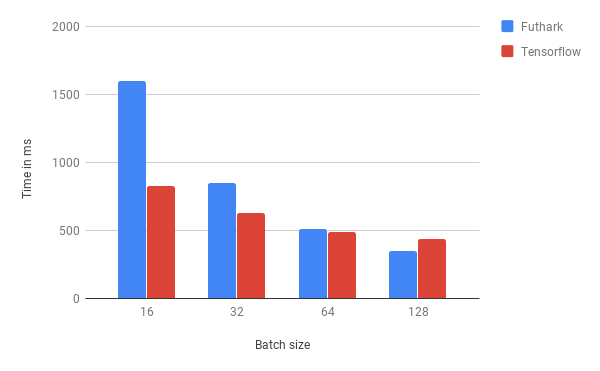
\includegraphics[width=\textwidth]{pics/MLPBenchmarkresults}
			\caption{Benchmark times (ms)}
		\end{subfigure}
		\begin{subfigure}[b]{0.49\textwidth}
			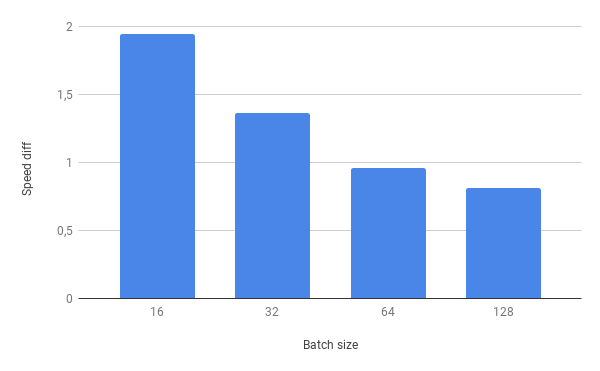
\includegraphics[width=\textwidth]{pics/Speedupmlp}	
			\caption{Relative speed diff.}
		\end{subfigure}
		\caption{Benchmark results for MLP}
		\label{fig:mlp}
	\end{figure}
	
	\section{Convolutional Network}
	The second benchmark is on the convolutional network used in the accuracy test. 
	The expectation are here lower than before, as we know that the implemented
	algorithm is not optimal for the convolutional layers. 
	The best that we can hope for are that Futhark is not orders of magnitudes
	slower. 
	The results are shown in Table \ref{tab:rescnn}
	\begin{table}[!h]
		\centering 
		\begin{tabular}{|l||*{5}{c|}}\hline
			\backslashbox{Library}{Batch size}
			&\makebox[3em]{16}&\makebox[3em]{32}&\makebox[3em]{64}&\makebox[3em]{128} 
			\\\hline\hline
			Tensorflow & $5881\ ms$ & $4168\ ms$ & $3343\ ms$ & $2748\ ms$\\\hline
			Futhark &  $12091 \ ms$ & $9010\ ms$ & $7992\ ms$ & $7515\ ms$   \\\hline
			\hline \Xhline{3\arrayrulewidth}  
			Relative speed diff. & 2.06 & 2.16 & 2.39 & 2.73 \\ \hline 
		\end{tabular}
		\caption{Benchmark results for convolutional network}
		\label{tab:rescnn}
	\end{table}\newline 
	The results show that for a batch size of 128, Futhark is 2.73 times slower than
	Tensorflow, but as the batch decreases the relative difference also shrinks,
	showing a similar results as \cite{Performance}, i.e. the GEMM approach works
	best at smaller batch sizes, but the performance are still relatively far from
	each other. 
	This is primarily due to that the GEMM approach doesn't perform better than the
	WMF or FFT algorithms on the filter sizes used in this network, even at smaller
	batch sizes. 
	\begin{figure}[!hbtp]
		\centering
		\begin{subfigure}[b]{0.49\textwidth}
			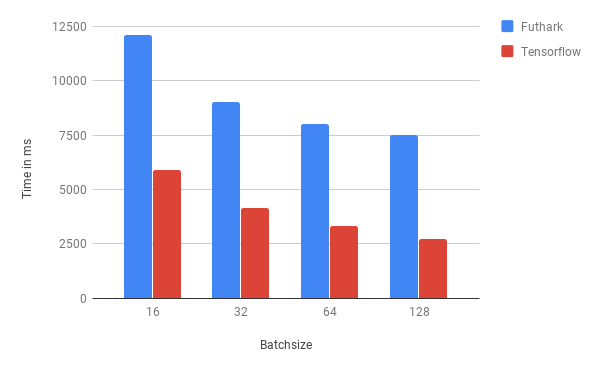
\includegraphics[width=\textwidth]{pics/ConvBenchmarkResults}
			\caption{Benchmark times (ms)}
			\label{fig:speed}
		\end{subfigure}
		\begin{subfigure}[b]{0.49\textwidth}
			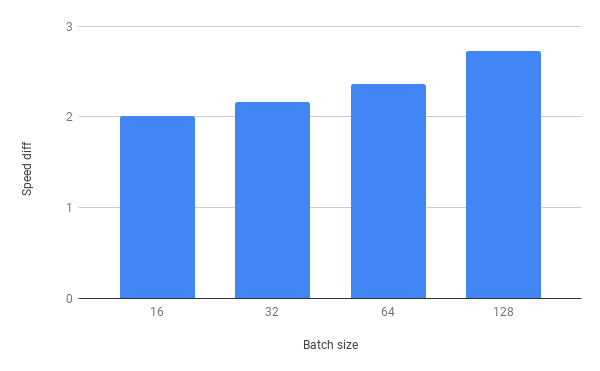
\includegraphics[width=\textwidth]{pics/speedupconv}	
			\caption{Relative speed diff.}
			\label{fig:mouse}
		\end{subfigure}
		\caption{Benchmark results for convolutional network}
		\label{fig:conv}
	\end{figure}
	
	\section{Reflection on results}
	To be able to reflect on the performance on the benchmark results, we should
	first try assess how fast Tensorflow is, in absolute terms.  S. Chintala
	\cite{benchmark} have benchmarked different convolutional networks with other
	popular libraries and shows that Tensorflow are among the fastest libraries, but
	is beaten by Torch\footnote{\url{http://torch.ch/}} and
	Neon\footnote{\url{https://ai.intel.com/neon/}}, though is Neon significantly
	faster on larger networks. 
	A comparison between Tensorflow and other cudNN based deep learning libraries in
	\cite{Performance} shows that they have similar in performance, when run in
	'benchmark' mode, meaning that they choose the best algorithms, either based on
	heuristics or simple brute-force. 
	Only Torch is a bit faster  in the paper. 
	While these results show that Tensorflow isn't the fastest it's clear that
	Tensorflow is not considered a slow library either as it is based on cudNN,
	which have been developed over multiple years, aiming at providing fast code for
	deep learning applications. 
	The fact that the benchmark shows similar or better performance for the MLP,
	where the underlying methods is the same, for a batch size of 64 and above is a
	great result. 
	The small gap on batch size of 32 is acceptable, but the large performance gap
	for a batch size of 16 is not so great, but one can argue that this result is
	less important, as this batch size is more uncommon than the others. 
	For the convolutional network, the benchmark results are clear; Tensorflow
	currently is the faster library, but we know that there is about a 2x
	performance gain in using better algorithms \cite{Performance}. 
	Assuming this, the library will be within a factor of 1.5 of Tensorflow, which
	would be a great accomplishment for a high-level language like Futhark. 
	Once those algorithms have been implemented, a more comprehensive comparison
	between those two will tell if the performance gap is only due to the choice of
	algorithms and if Futhark is capable of competing, in terms of performance, with
	Tensorflow. 
	Overall the benchmark results are promising for a deep learning library in
	Futhark, which eventually can perform at a similar level as Tensorflow. 
	Additionally as Futhark is a hardware independent language and thus cannot
	provide as much hardware specific optimizations as cudNN does, makes the
	benchmark results impressive, especially in the case of the MLP with a batch
	size of 128. 
	Considering that Futhark still is a relatively new, we can only expect that
	Futhark compiler will yield even better performance in the future as well.
	
